\chapter{The Standard Model and Beyond}
\label{chap:theory}

The Standard Model of particle physics describes all
known fundamental particles and the interactions between them (with the exception
of the gravitational force). Developed over decades in the latter half of the 20$^\mrm{th}$
century, it has predicted experimental findings to an extraordinary degree of accuracy,
and represents one of the crowning achievements of modern science.
However, despite it successes, there are a number of known phenomena that cannot be
explained with the current theory, giving physicists reason to look for an expanded model.
In this chapter, we outline the Standard Model as it currently exists, discuss some
of the challenges that the model faces, and give a brief summary of proposed extensions to
the Standard Model that are relevant to this dissertation.


\section{The Standard Model of particle physics}

The Standard Model (SM) is at its core a quantum field theory defined by a local 
$SU(3)\times SU(2)_L\times U(1)$ gauge symmetry. We will explain what exactly this means shortly 
(basically, each term gives rise to one of the three fundamental interactions), but for now we simply
describe all of the known particles and their properties.

\begin{figure}[ht]
  \begin{center}
    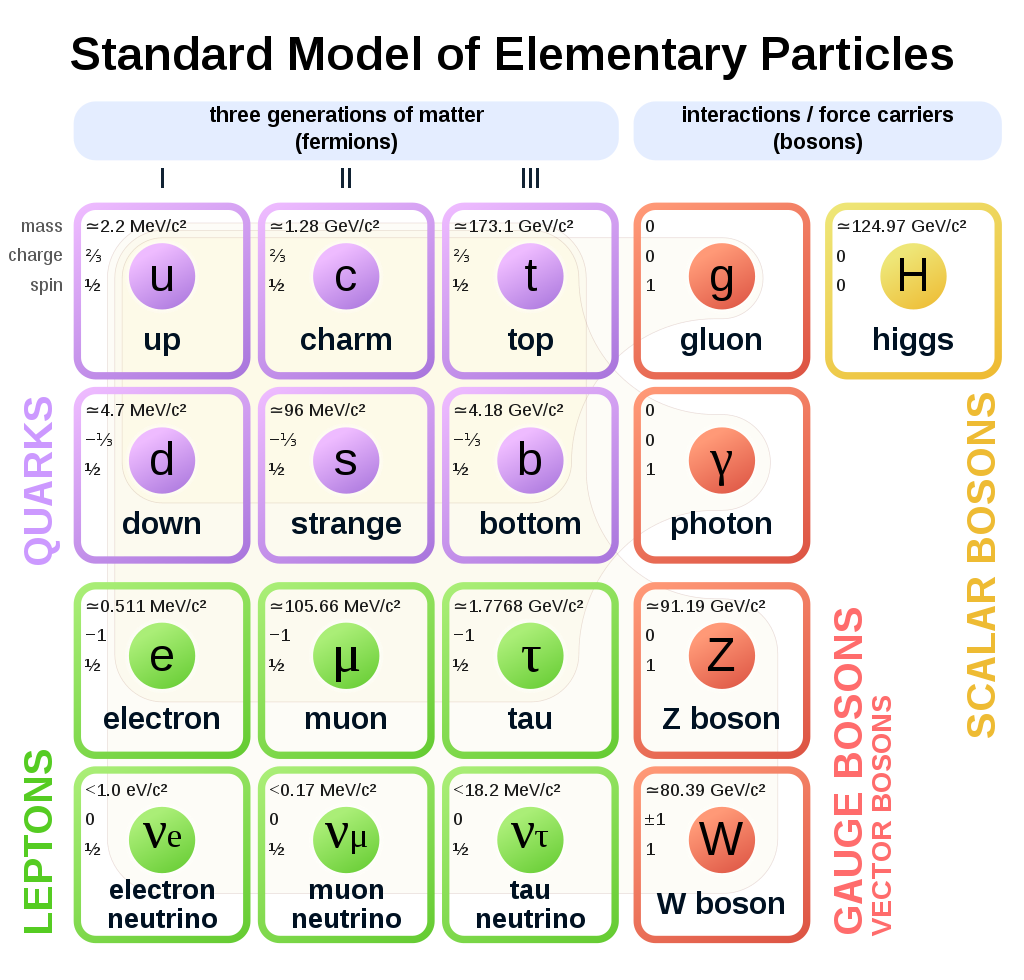
\includegraphics[width=0.70\textwidth]{figs/theory/standard_model.png}
    \caption{Diagram of all fundamental particles making up the Standard Model. There are 12 fermions (spin-\nicefrac{1}{2}), 
      consisting of six quarks (purple) and six leptons (green), 
      and divided into three generations. There are additionally four force-carrying vector bosons (spin-1),
      that couple to the fermions and give rise to the strong, weak, and electromagnetic interactions.
      Finally, the scalar Higgs boson, proposed in 1964 and discovered in 2012, provides the mechanism
      by which the other particles acquire mass. (Image from \cite{SM_diagram})
            }
    \label{fig:sm}
  \end{center}
\end{figure}

\subsection{Fundamental particles}

Figure~\ref{fig:sm} shows all distinct particles in the SM, organized into groups.
On the left, in purple and green, are the 12 fundamental fermions, defined by the
value of their intrinsic angular momentum, or ``spin'', of \nicefrac{1}{2} (in units
of $\hbar$). By the spin-statistics theorem, fermions obey the Pauli exclusion principle,
meaning no two can occupy the same quantum state simultaneously.

The fermions are further defined by the various charges they carry (which determine how they
interact with the bosons, as we will see). In green are the six leptons, three with electric charge
of $-1$ (electron, muon and tau) and three that are electrically neutral (electron neutrino, muon
neutrino, and tau neutrino). In purple are the 6 types of quarks. The up-type quarks (up, charm, and top)
have electric charges of $+2/3$, and the down-type quarks (down, strange, and bottom) have electric
charges of $-1/3$. The quarks, in contrast to the leptons, carry color charge, meaning they
can interact via the strong interaction. The color charge can be one of three values, typically
referred to as red, green, and blue.
All quarks and leptons carry weak isospin, meaning they can interact
via the weak interaction. Each of the fermions also has a corresponding antiparticle, which has the same
mass but opposite charges.

The fermions can be classified into three generations as indicated in the diagram, with masses
increasing in each generation. Due to various conservation laws arising from the allowed 
interactions, the first-generation particles are all stable, and hence form the building
blocks of matter. The strong interaction allows up and down quarks to strongly bind to
one another, forming protons (two ups and a down) and neutrons (two downs and an up).
The strong interaction further binds these into nuclei, which themselves bind to electrons via the electromagnetic
interaction to form atoms.

More generally, the strong interaction allows quarks to bind themselves into \textit{hadrons}, either in quark-antiquark
pairs called \textit{mesons}, or in three-quark configurations called \textit{baryons}. The net ``color content''
must be zero, which means mesons must contain e.g. a red quark and anti-red antiquark, and baryons
must contain exactly one red, blue, and green quark. The only stable baryon is the proton (the neutron
becomes stable when confined in a nucleus), and there are no stable mesons.

Moving to the right in the diagram, in red we have the four gauge bosons, which have spin-1
and which mediate the fundamental interactions. Their integer spin means they obey Bose statistics,
and are not constrained by the Pauli exclusion principle as are fermions. 
The gluon is massless, electrically neutral and mediates the strong
interaction. The photon is also massless and neutral and mediates the electromagnetic interaction. Finally,
the $W$ and $Z$ bosons are massive and mediate the weak interaction. The $Z$ is electrically neutral while 
the $W$ can carry charges of $\pm1$.

Finally, in yellow is the scalar (spin-0) Higgs boson. The Higgs mechanism was proposed in 1964 as an explanation
for how gauge bosons can acquire mass~\cite{Englert,Higgs,Guralnik}. A consequence of this mechanism is the prediction of a
scalar boson of undetermined mass, that couples to all SM particles proportionally to their masses.
The discovery of new boson of mass 125\GeV fitting these criteria (at least at the limits of current experimental precision) 
was announced by the CMS and ATLAS collaborations in July 2012~\cite{ATLAS:higgs,CMS:higgs}.

\subsection{Fundamental interactions}
\label{sec:fund_int}

Empirically, there are four known fundamental interactions, or ``forces'', between particles in our universe: 
the electromagnetic, weak, strong, and gravitational interactions. Gravity is understood
through Einstein's theory of general relativity, and is not (yet) integrated with our quantum understanding
of elementary particles. The other three interactions, on the other hand, are mathematically described by the
SM.

Essentially, each of the interactions arises by requiring that the Lagrangian describing the particle dynamics is
invariant under a certain \textit{local gauge transformation}. This means that if the particle fields are transformed
by some function that depends on spacetime position $x$, the Lagrangian is unchanged.
The full details are given in any quantum field theory textbook (e.g.~\cite{Peskin}), and we just give a brief
summary of the main ideas here.

The simplest example is the electromagnetic interaction. Starting with the Lagrangian of a free fermion
\be\label{eq:ferm_lagr}
\mathcal{L}_\mrm{fermion} = i\bar{\psi}\gamma^\mu\partial_\mu\psi - m\bar{\psi}\psi,
\ee
where $\psi$ is the spinor field of the fermion and $m$ is its mass,
we require that $\mathcal{L}$ is invariant under the local $U(1)$ transformation $\psi\to e^{-iq\theta(x)}\psi$.
The Lagrangian in Eq.~\ref{eq:ferm_lagr} is \textit{not} invariant under this transformation,
as we are left with an extra term proportional to $\partial_\mu\theta(x)$.

It turns out we can fix this by adding an extra term $-q\bar{\psi}\gamma^\mu\psi A_\mu$, where
$A_\mu$ is a new vector field that transforms by $A_\mu\to A_\mu+\partial_\mu\theta$. The new terms
introduced by the gauge transformation then cancel, and the Lagrangian is invariant.  The field
$A_\mu$ represents a new spin-1 particle, and to ensure that the Klein-Gordon equation is satisfied,
we must also add a ``free'' term. Doing this, it turns out the boson must be massless to ensure gauge invariance is
maintained.

So by requiring that the Lagrangian for a free fermion is invariant under a local $U(1)$ transformation,
we were forced to introduce a new massless, spin-1 boson that couples to the fermion via the term
$q\bar{\psi}\gamma^\mu\psi A_\mu$. This new boson is the photon, and this fermion coupling
is the fundamental interaction of quantum electrodynamics (QED)! The photon couples to any particle with
electric charge, represented by $q$ in the coupling term.

Feynman diagrams for the fundamental vertices of QED are shown in Fig.~\ref{fig:em_diagrams}.
On the left is the coupling of the photon to any charged fermion (leptons, with $|q|=1$, or
quarks, with $|q|=2/3$ or 1/3). The $W$ boson is also charged, and so couples to the photon,
but this vertex is best understood through electroweak unification discussed below.


\begin{figure}[t]
  \addtolength{\abovecaptionskip}{5mm}
  \centering
  \vskip5mm
  \begin{fmffile}{feynman_diagrams/em_ferm}
  \begin{fmfgraph*}(40,25)
    \fmfleft{v1}
    \fmfright{o1,o2}
    \fmflabel{$e^-$}{o1}
    \fmflabel{$e^+$}{o2}
    \fmf{fermion}{o1,v2,o2}
    \fmf{photon,label=$\gamma$}{v1,v2}
  \end{fmfgraph*}
\end{fmffile}

  \begin{fmffile}{feynman_diagrams/em_w}
  \begin{fmfgraph*}(40,25)
    \fmfleft{v1}
    \fmfright{o1,o2}
    \fmflabel{$W-$}{o1}
    \fmflabel{$W+$}{o2}
    \fmf{boson}{o1,v2,o2}
    \fmf{photon,label=$\gamma$}{v1,v2}
  \end{fmfgraph*}
\end{fmffile}

  \caption{Fundamental vertices of the electromagnetic interaction. The photon couples to charged fermions (left)
    and the $W$ boson (right), though the $\gamma WW$ vertex is best understood through electroweak
    unification discussed later in this section.
  }
  \label{fig:em_diagrams}
\end{figure}

To derive the strong interaction, we start with the assumption that quarks have ``color charge'',
which can be one of three values we refer to as red, green, and blue.
Then the free quark Lagrangian can be written
\be\label{eq:quark_lagr}
\begin{split}
\mathcal{L}_\mrm{quarks} &= \sum_{c=r,g,b} i\bar{q}_c\gamma^\mu\partial_\mu q_c - m\bar{q}_c q_c \\
&= i\bar{q}\gamma^\mu\partial_\mu q - m\bar{q}q
\end{split}
\ee
where $q$ is the quark spinor, $c$ represents the color charge, and we have introduced the shorthand
\be
q = \begin{pmatrix} q_r \\ q_g \\ q_b \end{pmatrix}, \;\;\;
\bar{q} = \left( \bar{q}_r \; \bar{q}_g \; \bar{q}_b \right).
\ee
This can also be summed over
the six flavors of quarks to describe all of them simultaneously.

The Lagrangian in Eq.~\ref{eq:quark_lagr} is already invariant under the global gauge transformation
$q\to Uq$, where $U$ is any $3\times3$ unitary matrix of determinant 1 (this group of matrices is called
$SU(3)$. It is not strictly necessary to require determinant 1, but we can factor out the determinant
as a separate $U(1)$ transformation, which would just re-derive QED for quarks). But if we further require
that the theory should be invariant under a \textit{local} $SU(3)$ transformation $U(x)$, we are again required
to add extra terms.

The details are quite a bit messier this time, as $SU(3)$ is a non-abelian group. But it turns out
that any matrix in $SU(3)$ can be written as $e^{-ig_s\boldsymbol\lambda\cdot\boldsymbol\alpha(x)}$, where
$\boldsymbol\lambda$ are the eight Gell-Man matrices and $\boldsymbol\alpha$ is an 8-dimensional vector,
and we are forced to add a term to the Lagrangian $g_s\bar{q}\gamma^\mu\boldsymbol(\boldsymbol\lambda\cdot\mathbf{A_\mu})q$.

This time, $\mathbf{A_\mu}$ is a vector of eight new spin-1 bosons (gluons), and this term represents the coupling of gluons
to quarks. In adding the kinetic terms for the gluons, we are again forced to make them massless, but this time,
due to the non-abelian nature of $SU(3)$, we are also forced to add additional terms that represent three- and four-gluon 
self-interaction vertices. The fundamental interactions for quantum chromodynamics (QCD) are shown in Fig.~\ref{fig:strong_diagrams}.
The two on the right are the boson self-interactions, which are not present in QED, and are a feature of non-abelian
gauge theories.

\begin{figure}[t]
  \addtolength{\abovecaptionskip}{5mm}
  \centering
  \vskip5mm
  \begin{fmffile}{feynman_diagrams/glu_q}
  \begin{fmfgraph*}(40,25)
    \fmfleft{v1}
    \fmfright{o1,o2}
    \fmflabel{$\bar{q}_j$}{o1}
    \fmflabel{$q_i$}{o2}
    \fmflabel{$g$}{v1}
    \fmf{fermion}{o1,v2,o2}
    \fmf{gluon}{v1,v2}
  \end{fmfgraph*}
\end{fmffile}

  \begin{fmffile}{feynman_diagrams/glu_tri}
  \begin{fmfgraph*}(40,25)
    \fmfleft{v1}
    \fmfright{o1,o2}
    \fmflabel{$g$}{o1}
    \fmflabel{$g$}{o2}
    \fmflabel{$g$}{v1}
    \fmf{gluon}{o1,v2,o2}
    \fmf{gluon}{v1,v2}
  \end{fmfgraph*}
\end{fmffile}

  \begin{fmffile}{feynman_diagrams/glu_quad}
  \begin{fmfgraph*}(40,25)
    \fmfleft{i1,i2}
    \fmfright{o1,o2}
    \fmflabel{$g$}{i1}
    \fmflabel{$g$}{i2}
    \fmflabel{$g$}{o1}
    \fmflabel{$g$}{o2}
    \fmf{gluon}{i1,v1,i2}
    \fmf{gluon}{o1,v1,o2}
  \end{fmfgraph*}
\end{fmffile}

    \caption{Fundamental vertices of the strong interaction. The gluon couples to a quark-antiquark
      pair, and also has 3- and 4-gluon self-interaction vertices. These are important for internal
      dynamics of hadrons as well as the hadronization of quarks and gluons at colliders.
            }
    \label{fig:strong_diagrams}
\end{figure}

The final interaction we must incorporate is the weak interaction. However, there are a number of difficulties
that did not arise for the electromagnetic and strong interactions. First is the observation that charged weak
currents (that is, $W$ boson interactions), only involve left-handed chiral fermions states, 
or right-handed anti-fermion states (in the relativistic
limit, or for massless particles, chirality is the same as helicity). The strong and electromagnetic
interactions make no distinction between left- and right-handed states. 

This is incorporated into the theory
by introducing left-handed fermion doublets (e.g. $(\nu_e\;e)_L$, $(u\;d)_L$, etc.) and right-handed
singlets, and then imposing a local $SU(2)$ symmetry on the doublet states. The charge corresponding
to this symmetry is called \textit{weak isospin}.

Running through the same procedure as above, we find that this $SU(2)_L$ symmetry generates
two charged currents and one neutral current, which look deceivingly like the $W^\pm$ and $Z$
bosons. However, there is a problem: the neutral $Z$ boson is observed to couple to both left-
and right-handed particles, while so far we have only dealt with the left-handed case.

The answer to this is tied to the solution for the other main problem of weak interactions: the fact that
the weak bosons are massive. We have seen that local gauge invariance requires that the gauge bosons
be massless, but in reality the weak gauge bosons are observed to be quite heavy. The solution
to this in general was provided by the Higgs mechanism, mentioned above and discussed in the following.
Then in the late 1960s, Glashow, Weinberg, and Salam~\cite{Glashow,Weinberg,Salam} incorporated this into
the SM and in the process unified the electromagnetic and weak interactions into a single
\textit{electroweak} interaction.

Before getting into the Higgs mechanism, we can understand this unification by introducing a 
\text{weak hypercharge}, defined as $Y=2T_3-2Q$, where $Q$ is the electric charge and
$T_3$ is the third (neutral) component of weak isospin. This is an invariant quantity
under weak isospin and the total symmetry group becomes $SU(2)_L\times U(1)$.
Denoting $\mathbf{j_\mu}$ and $j^Y_\mu$ as the four currents associated with weak isospin
and weak hypercharge, respectively, the electroweak interaction Lagrangian can be written
\be\label{eq:ew_lagr}
\mathcal{L}_\mrm{EWK, int} = -ig_w\mathbf{j_\mu}\cdot \mathbf{W}^\mu + \frac{ig'}{2}j^Y_\mu B^\mu,
\ee
where we have introduced coupling constants $g_w$ and $g'$. This is written in terms
of the \textit{gauge fields} rather than the \textit{physical fields}, to make it more
manifestly invariant under our symmetry group, but it can be re-written in terms of
the physical fields. The two $W$ bosons are linear combinations of the first two 
(charged) components of $\mathbf{W_\mu}$, and the $Z$ boson and photon are linear combinations
of $W_\mu^3$ and $B_\mu$:
\be\label{eq:wpm}
W_\mu^\pm = \frac{1}{\sqrt{2}}(W^1_\mu \mp iW^2_\mu)
\ee
\be\label{eq:za}
\begin{pmatrix} A_\mu \\ Z_\mu \end{pmatrix} = 
\begin{pmatrix} \cos\theta_w & \sin\theta_w \\ -\sin\theta_w & \cos\theta_w \end{pmatrix}
\begin{pmatrix} B_\mu \\ W^3_\mu \end{pmatrix},
\ee
where $\theta_w$ is a free parameter that controls the degree of mixing, known as the 
Weinberg angle or weak mixing angle

From these and the known QED coupling, one can derive expressions for the weak coupling
constants $g_w$ and $g'$ in terms of $e$ and $\theta_w$. Plugging Eqs.~\ref{eq:wpm}
and \ref{eq:za} into the Lagrangian Eq.~\ref{eq:ew_lagr}, one can get an expression
for the Lagrangian in terms of the physical fields and read off the allowed couplings.
The fundamental vertices are shown in Fig.~\ref{fig:weak_diagrams}. The $W$ couples
to $\ell\nu$ or $q\bar{q}'$ pairs (though only to left-handed fermions
and right-handed antifermions). The $\ell\nu$ pair must be within a single generation,
but cross-generational $q\bar{q}'$ couplings are possible as the \textit{weak eigenstates}
of quark flavor are rotated slightly from the \textit{mass eigenstates} that we have been
referring to. The matrix that performs this rotation and determines the coupling strengths
is known as the CKM matrix.
The $Z$ couples to any fermion-antifermion pair.

\begin{figure}[t]
  \addtolength{\abovecaptionskip}{5mm}
  \centering
  \vskip5mm
  \begin{fmffile}{feynman_diagrams/w_lep}
  \begin{fmfgraph*}(40,25)
    \fmfleft{v1}
    \fmfright{o1,o2}
    \fmflabel{$\bar{\nu}_\ell$}{o1}
    \fmflabel{$\ell^-$}{o2}
    \fmf{fermion}{o1,v2,o2}
    \fmf{photon,label=$W^-$}{v1,v2}
  \end{fmfgraph*}
\end{fmffile}

  \begin{fmffile}{feynman_diagrams/w_q}
  \begin{fmfgraph*}(40,25)
    \fmfleft{v1}
    \fmfright{o1,o2}
    \fmflabel{$\bar{q}_j$}{o1}
    \fmflabel{$q_i$}{o2}
    \fmf{fermion}{o1,v2,o2}
    \fmf{photon,label=$W$}{v1,v2}
  \end{fmfgraph*}
\end{fmffile}

  \begin{fmffile}{feynman_diagrams/z_ferm}
  \begin{fmfgraph*}(40,25)
    \fmfleft{v1}
    \fmfright{o1,o2}
    \fmflabel{$\bar{f}$}{o1}
    \fmflabel{$f$}{o2}
    \fmf{fermion}{o1,v2,o2}
    \fmf{photon,label=$Z$}{v1,v2}
  \end{fmfgraph*}
\end{fmffile}

    \caption{Fundamental vertices of the weak interaction. The $W$ boson can couple to a lepton
      and a same-generation neutrino, or a quark and anti-quark (most strongly within the same
      generation, but cross-generational couplings are possible via the CKM matrix).
      The $Z$ boson can couple to any fermion and its antiparticle. There are also
      boson self-interaction vertices ($WWZ$, $WWWW$, $WWZZ$, $\gamma\gamma WW$) necessary for the self-consistency 
      of the theory, but they are less important practically.
            }
    \label{fig:weak_diagrams}
\end{figure}

We have seen how the electromagnetic, strong, and weak interactions can arise by imposing
a local $SU(3)\times SU(2)_L\times U(1)$ gauge symmetry on the SM Lagrangian.
However, there remain the questions of how exactly the weak bosons acquire their masses without breaking
local gauge invariance, and how the $SU(2)_L\times U(1)$ symmetry underlying the electroweak
interaction is broken, such that the weak bosons are so heavy while the photon is massless.

The answer lies in the Higgs mechanism and spontaneous symmetry breaking, mentioned earlier.
Again the details can be found in any quantum field theory textbook, but the basic idea is this:
imagine that there exists a scalar complex field $\phi\equiv\phi_1+i\phi_2$ governed by the Lagrangian
\be
\mathcal{L} = \frac{1}{2}\partial_\mu\phi^*\partial_\mu\phi + \frac{1}{2}\mu^2\phi^*\phi - \frac{1}{4}(\phi^*\phi)^2.
\ee

This  Lagrangian already has a global $U(1)$ symmetry, and requiring local symmetry again requires the addition
of a massless gauge boson $A_\mu$.
Further, the potential (given by the negative of the final two terms) normally has a minimum at 0, but in this case 0 is
actually a local maximum and the minimum lies on a circle in the complex plane of radius $\mu/\lambda$.
Since the Feynman calculus is really a perturbation theory in the fields, we must expand around a local minimum of the
potential. Choosing $(\mu/\lambda,0)$ as the point to expand around (``spontaneously'' breaking the symmetry), we define
\be
\eta\equiv\phi_1-\mu/\lambda, \;\;\; \xi\equiv\phi_2.
\ee

Plugging these in to the Lagrangian, we find that $\eta$ represents a scalar boson of mass $m_\eta=\sqrt{2}\mu$,
and $A_\mu$ picks up a mass term $m_A=2q\mu/\lambda$, where $q$ is the charge generated by the $U(1)$
symmetry. So by introducing a complex scalar field and breaking the symmetry of its potential, we have given
mass to the gauge boson at the cost of a new scalar boson $\eta$! There is a problematic term representing
a direct $\xi A$ coupling, but this can be transformed away with the proper choice of gauge, thereby eliminating 
the non-physical ``Goldstone boson'' $\xi$.

It is a bit more complicated with the full $SU(2)_L\times U(1)$ symmetry of the electroweak Lagrangian (the scalar
field must become a doublet of complex fields, and we have three gauge bosons), but the basic ideas are the same.
We find that the $W$ and $Z$ bosons acquire masses proportional to $\mu/\lambda$ (and related by $M_W/M_Z=\cos\theta_W$)
while the photon remains massless, and a new scalar ``Higgs boson'' is introduced. Its mass is undetermined by the theory
and must be measured.

Masses of the fermions can also be added to the theory via the Higgs boson, by adding Yukawa coupling terms. We then get all of the fundamental
interactions of the Higgs boson shown in Fig.~\ref{fig:higgs_diagrams}. It directly couples to all massive particles,
with strength proportional to the mass. While it does not directly couple to photons or gluons as they are massless,
the Higgs can still decay to these particles through loops involving massive particles (most prominently
virtual top quarks).

\begin{figure}[t]
  \addtolength{\abovecaptionskip}{5mm}
  \centering
  \vskip5mm
  \begin{fmffile}{feynman_diagrams/higgs_ferm}
  \begin{fmfgraph*}(40,25)
    \fmfleft{v1}
    \fmfright{o1,o2}
    \fmflabel{$\bar{f}$}{o1}
    \fmflabel{$f$}{o2}
    \fmf{fermion}{o1,v2,o2}
    \fmf{dashes,label=$H$}{v1,v2}
  \end{fmfgraph*}
\end{fmffile}

  \begin{fmffile}{feynman_diagrams/higgs_boson}
  \begin{fmfgraph*}(40,25)
    \fmfleft{v1}
    \fmfright{o1,o2}
    \fmflabel{$W,Z$}{o1}
    \fmflabel{$W,Z$}{o2}
    \fmf{boson}{o1,v2,o2}
    \fmf{dashes,label=$H$}{v1,v2}
  \end{fmfgraph*}
\end{fmffile}

  \begin{fmffile}{feynman_diagrams/higgs_gamma}
  \begin{fmfgraph*}(40,25)
    \fmfleft{v1}
    \fmfright{o1,o2}
    \fmflabel{$\gamma,g$}{o1}
    \fmflabel{$\gamma,g$}{o2}
    \fmf{fermion}{v2,v3,v4,v2}
    \fmf{photon}{v3,o1}
    \fmf{photon}{v4,o2}
    \fmf{dashes,label=$H$}{v1,v2}
  \end{fmfgraph*}
\end{fmffile}

    \caption{Interactions of the Higgs boson. It directly couples to any particle with mass,
      including fermions (left) and the $W$ and $Z$ bosons (middle). It cannot couple directly
      to massless particles such as the photon and gluon, but it may decay to these through loops
      of massive particles (right). The most likely particle in the loop is the top quark, since
      it is the heaviest option (thought it needs to be virtual, since $2m_t > m_H$). There
      are also three- and four-Higgs self-interaction vertices.
            }
    \label{fig:higgs_diagrams}
\end{figure}

We have now seen the basic ideas of how the Standard Model is constructed: starting from the Lagrangians
of free fermions, we impose invariance under local $SU(3)\times SU(2)_L\times U(1)$ gauge transformations
and are forced to add massless gauge bosons. By introducing a scalar Higgs field, we can spontaneously 
break the symmetry of the electroweak interaction and give masses to the weak bosons, as well as
give mass terms to the fermions in the theory. The resulting theory has had remarkable success in
predicting experimental findings to high degree of accuracy. However, there are a number of phenomena
that the SM cannot explain, and it thus cannot be a complete ``theory of everything''. We examine some
of the issues with the SM in the following section.


\section{Shortcomings of the Standard Model}
The Standard Model has a long history of making successful predictions about the sub-atomic
world: the existence of the charm and top quarks, gluons, the weak bosons, and the Higgs boson;
branching ratios and lifetimes of the fundamental particles and hadrons; the precise value of the
electron's anomalous magnetic moment (down to one part in a billion, making it one of the most accurate
verified prediction in the history of physics); and more. Many experiments continue today to verify the SM's
accuracy. However, it is not a perfect theory and cannot sufficiently explain a number of observed
phenomena.

\subsection{Unexplained phenomena and theoretical considerations}

First and foremost among unexplained phenomena is the gravitational interaction. 
The SM provides a mathematical framework to describe
three out of the four known fundamental interactions, but does not say anything about the mutual attraction
of massive particles. Instead, gravitation is currently understood in terms of curvature of spacetime
through Einstein's general theory of relativity. This is incompatible with our present understanding of
particle physics, and the search for a quantum theory of gravity remains an active area
of research among theoretical physicists.

The SM does not naturally allow for neutrino masses (the Yukawa mechanism for adding masses to the charged leptons
requires the existence of right-handed leptons, but only left-handed neutrinos have been observed). However,
experiments have observed the phenomenon of ``neutrino oscillation''~\cite{PDGreview14}, whereby a neutrino that
starts as one flavor (e.g. an electron neutrino) is later measured after some propagation as a different flavor
(e.g. a muon neutrino). This is only possible if the mass eigenstates of neutrinos are rotated from the flavor
eigenstates that are produced in weak interactions, which necessarily requires that the neutrinos have small
but non-zero masses. It is possible to modify the SM to incorporate neutrino masses, but such solutions are
unsatisfactory as they offer no insight into the vastly different scales of neutrino and charged fermion masses.
Theorists seek a more natural explanation for the origin of neutrino masses.

Another problem lacking a satisfactory explanation under the SM is that of matter-antimatter asymmetry, 
or the ``baryon asymmetry''~\cite{Canetti:baryon_asymm}. 
We observe that the universe is made almost entirely out of matter, as opposed
to antimatter, and there is no good reason that this should be the case (the SM predicts that almost equal amounts
of matter and antimatter should have been created at the beginning of the universe, after which most of it
would have been annihilated). A necessary condition for explaining this asymmetry is a mechanism for violating
charge-parity, or CP, symmetry (the symmetry that exchanges all particles for antiparticles and reverses chiralities).
The weak interaction allows for small CP-violation via a complex phase in the CKM quark mixing matrix, but this
is not big enough to explain the observed baryon asymmetry, so beyond the SM sources are necessary.

Finally, most relevant for this dissertation is the existence of \textit{dark matter}. If one plots the velocity of
matter as a function of radial distance from the center in a rotating spiral galaxy, Newton's laws
applied to the distribution of visible matter say that the velocity should decrease with radius. However, observed 
galactic rotation curves are actually flat over large distances (see Fig.~\ref{fig:dm_curve} for an example from the M33
galaxy). This suggests the presence of invisible, or ``dark'', matter permeating the galaxies that interacts
gravitationally but not electromagnetically. Other observations support this same hypothesis, such as gravitational
lensing and the cosmic microwave background power spectrum. The SM does not provide for any fundamental particles
that can account for this dark matter, and explaining it is one of the central problems of modern physics.

\begin{figure}[t]
  \centering
  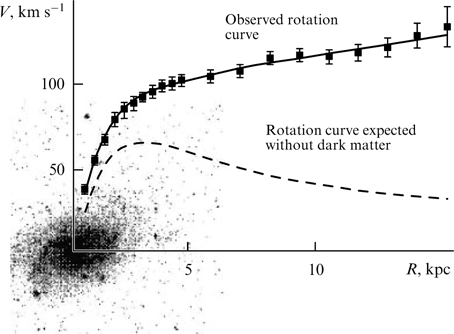
\includegraphics[width=0.5\textwidth]{figs/theory/dm.jpg}
  \caption{Observed and expected rotation curves of the M33 galaxy, suggesting
    a significant mass contribution from dark matter. (Image from~\cite{Zasov:dm})
            }
    \label{fig:dm_curve}
\end{figure}

There are also a few problems with the SM that are more theoretical in nature and motivated by ``naturalness'' concerns.
That is, that the parameters of the SM are ``fine-tuned'' to specific values for no apparent reason (e.g. an underlying symmetry
that would cause the parameter to take on that value). Extensions to the SM are sought that would provide more 
natural explanations.

One example is known as the ``strong CP problem''. As mentioned above, the weak sector admits slight CP symmetry violation
via a complex phase in the CKM quark mixing matrix. It is also possible to add CP-violation to the strong sector, but this
is not observed experimentally. This means that the parameter controlling this CP-violating term in the QCD Lagrangian
must be very close to 0. There is no known reason for this, and theorists have provided a number of models that can explain
it more naturally. However, no evidence for any of these theories has yet been found experimentally.

Finally, with what will partially motivate the kinds of new physics sought in the present analysis, we have what is known as the
``hierarchy problem.'' The observed Higgs mass of 125\GeV is the sum of the ``bare Higgs mass'', a free parameter in the theory,
plus terms arising from loop-level corrections to the free propagator. The most important of these corrections is shown in
Fig.~\ref{fig:higgs_massloop}. As the Higgs couples to all massive fermions, the virtual particle loop can be anything. The most
important contribution however is from the top quark, since the top quark is the heaviest particle and couples most strongly to
the Higgs. Computing amplitudes, one finds (to leading order in $\Lambda$)
\be\label{eq:higgsmass}
m_{H,\mrm{obs}}^2 \approx m_{H,\mrm{bare}}^2 - \frac{|\lambda|^2}{8\pi^2}\Lambda^2,
\ee
where $\lambda$ is the top quark Yukawa coupling and $\Lambda$ is the scale up to which the 
SM is valid, typically taken to be the Planck scale $\Lambda\approx 10^{19}\GeV$.

\begin{figure}[t]
  \addtolength{\abovecaptionskip}{2mm}
  \centering
  \begin{fmffile}{feynman_diagrams/higgs_massloop}
  \begin{fmfgraph*}(40,25)
    \fmfleft{i1}
    \fmfright{o1}
    \fmf{fermion,left,tension=0.4,label=$t$}{v1,v2,v1}
    \fmf{dashes}{i1,v1}
    \fmf{dashes}{v2,o1}
    \fmflabel{$H$}{i1}
    \fmflabel{$H$}{o1}
  \end{fmfgraph*}
\end{fmffile}

    \caption{Diagram representing the loop-level correction to the Higgs mass. The loop
      can be any charged fermion, but the top quark is most important since it has the highest mass.
            }
    \label{fig:higgs_massloop}
\end{figure}

Now the observed Higgs mass is of order $m_{H,\mrm{obs}}^2\sim 10^4\GeV^2$, and the correction
term is of order $10^{36}\GeV^2$. That means that the unobservable bare Higgs mass must be fine-tuned to
one part in $\sim10^{32}$ in order to cancel the correction almost perfectly, and there is no
reason why this must be so. In other words, we ask
\textit{why is the Higgs mass so much smaller than the Planck scale?}
The fact that this must be a complete accident in the SM is highly unnatural, and leads to the question
of whether there is some kind of physics beyond the SM that could provide a more satisfactory explanation.

\subsection{Signs of experimental deviation}
\label{sec:exp_dev}

While the SM has been extensively tested and probed to astounding degrees of accuracy, there are have
been a few signs of deviation between theory and experimental results. Many of these have come and gone
over the years, shown to be merely statistical fluctuation, but a small number remain open questions today.

First is the anomalous magnetic moment of the muon. Particles with intrinsic spin also have an intrinsic
magnetic moment caused by that angular momentum. The dimensionless proportionality constant
relating this moment to the particle's spin and the Bohr magneton is known as the ``$g$-factor''.
In ordinary quantum mechanics, this is exactly equal to 2 for fermions such as the electron and muon.
However, QED predicts small corrections to this from virtual particle loops. The $g$-factor
of the electron has been measured as $g_e=2.002\;319\;304\;361\;46(56)$~\cite{Hanneke:eleg2}, agreeing with theory to around
one part in $10^{10}$ and making it one of the most precisely verified predictions in all of physics.

The muon $g$-factor has been measured to around 1 part in $10^6$, but is higher than the predicted theory value by 3--4
standard deviations~\cite{Blum:muong2}. There are various models of beyond the SM physics that could in principle explain
this, but it is still an open question whether the discrepancy is due to new physics, statistical
fluctuation, or poorly modeled experimental or theoretical uncertainties. The Muon $g-2$ experiment at Fermilab
is currently taking data and should reduce the experimental uncertainty by more than a factor of 3.

Second is a collection of flavor physics anomalies in the decays of $B$ mesons~\cite{Graverini:flavour}. 
The SM predicts the principle of
\textit{lepton flavor universality} (LFU), which states that the three generations of leptons are identical in all but
their  masses (i.e., their couplings to the electroweak bosons are the same). New particles could in principle
couple differently to different generations, changing branching fractions for mesons that decay via
the weak interaction into leptons. The BaBar, Belle, and LHCb collaborations have measured the ratios
\be
R_{D^{(*)}} = \frac{\mrm{Br}(B\to D^{(*)}\tau\bar{\nu}_\tau)}{\mrm{Br}(B\to D^{(*)}\ell\bar{\nu}_\ell)}, \;\;\;\;\;
\text{with } \ell=\mu,e
\ee
and have found values consistently higher than the SM predictions, with the averages being 2--3 standard deviations
larger than the SM values. Fig.~\ref{fig:b_anomalies} shows the measured averages compared to SM expectations.

\begin{figure}[t]
  \centering
  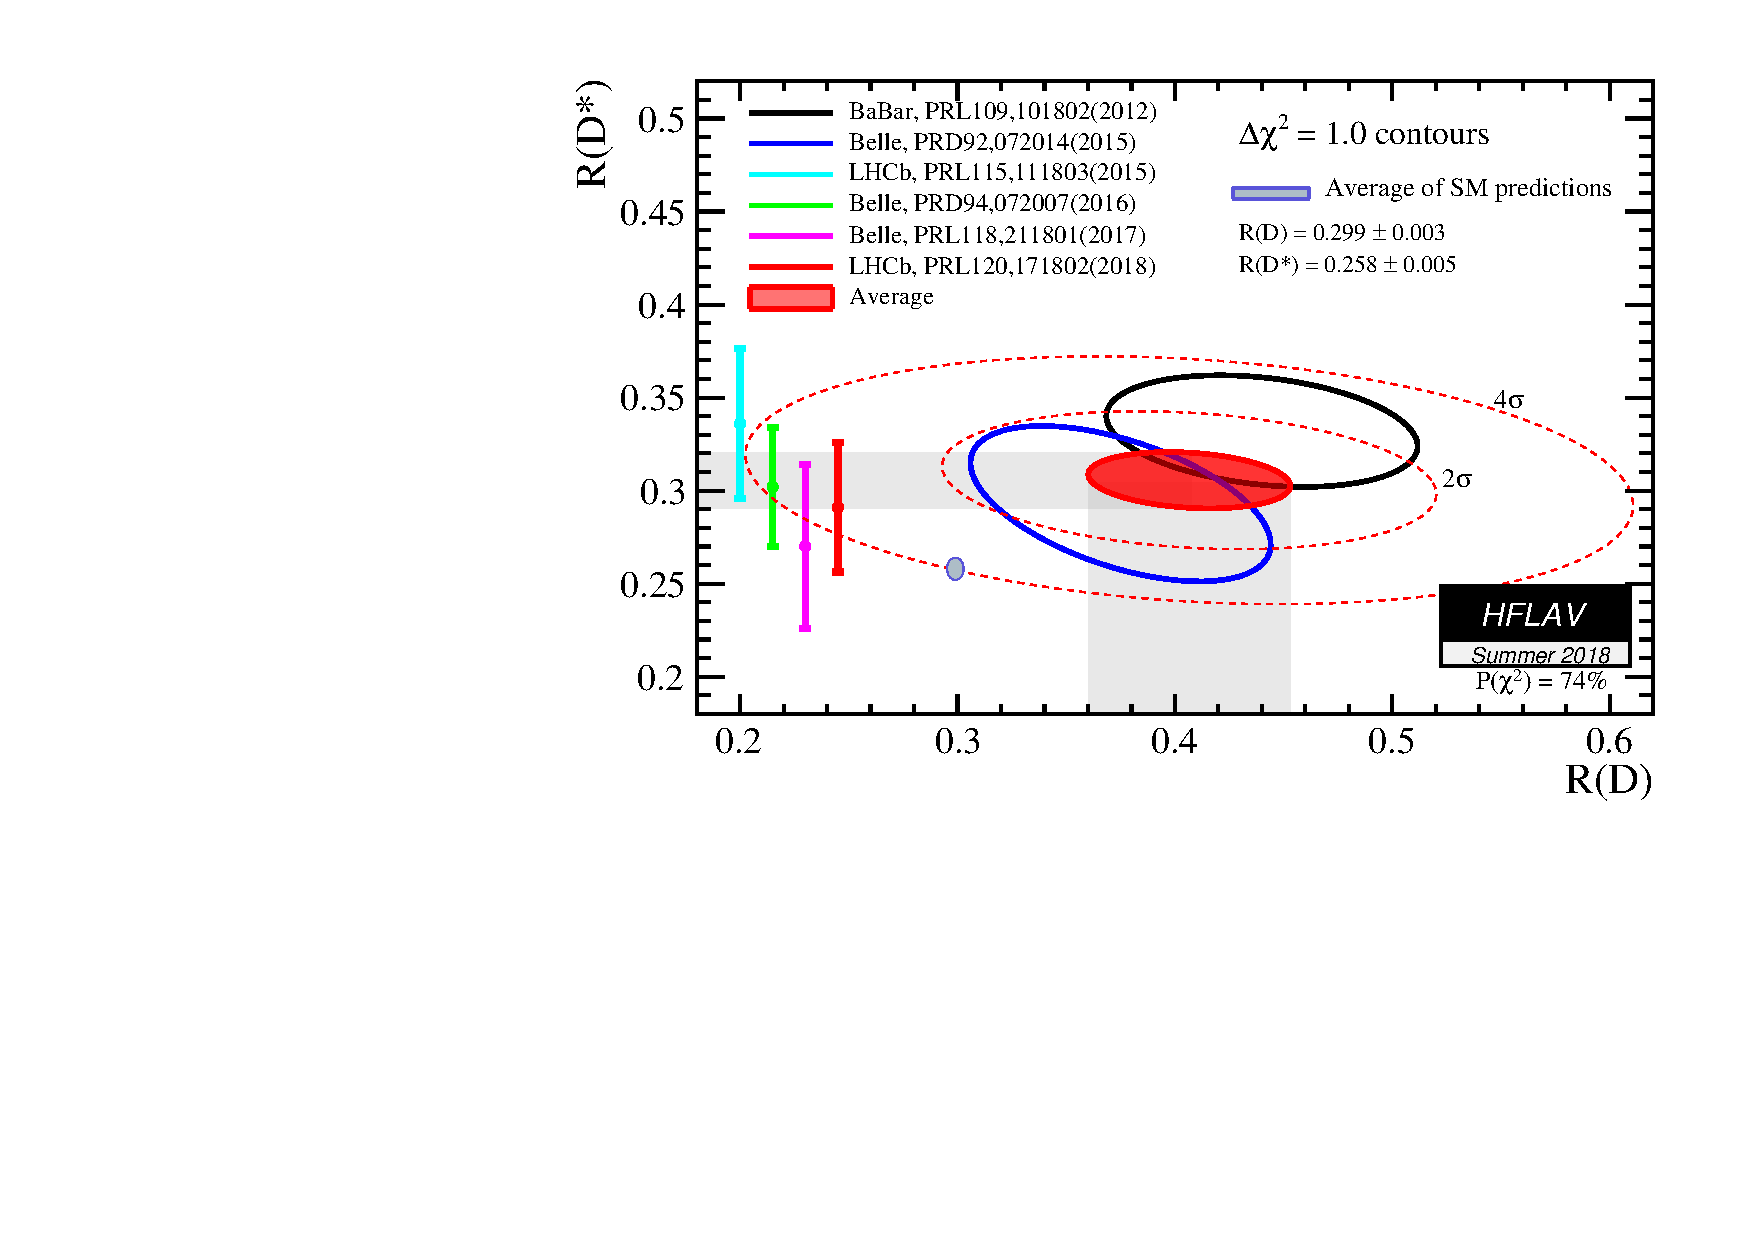
\includegraphics[width=0.6\textwidth]{figs/theory/b_anomalies.pdf}
  \caption{Averages of $R_D$ and $R_{D^*}$ as measured by the BaBar, Belle, and LHCb Collaborations.
    Both ratios are 2--3 standard deviations higher than the SM expectation. (Image from~\cite{HFLAV})
            }
    \label{fig:b_anomalies}
\end{figure}

The experiments have also probed LFU via the rarer loop-level neutral current $b\to s\ell\ell$ processes,
in the form of $R_{K^{(*)}} = \mrm{Br}(B\to K^{(*)}\mu^+\mu^-) / \mrm{Br}(B\to K^{(*)}e^+e^-)$. This shows similar
$2\sigma$-level deviation from the SM prediction. Analysis of data from LHCb and the recently started Belle 2 run
should improve the experimental precision and give a clearer picture of whether or not the anomalies are real.

\section{Theories of physics beyond the Standard Model}
\label{sec:bsm}
There is a huge variety of models of physics beyond the SM (BSM), each with their own predictions of new particles
and phenomena. The list is far too vast and diverse to summarize completely here, so we only discuss briefly the ones most
relevant to the analysis presented in this dissertation.

\subsection{Supersymmetry}
\label{sec:susy}

Supersymmetry (SUSY) is a proposed extension to the SM dating to the 1970s that posits that every SM fermion has a bosonic 
``superpartner'', and every SM boson has a fermionic superpartner. 
While a theory that doubles the number of fundamental particles and adds over 100 parameters to the SM
is not the most elegant of solutions, it has become popular
as it can solve the hierarchy problem and provide a natural candidate for dark matter.
We give a brief overview of the main ideas here;
a more complete summary can be found at \cite{SUSYprimer}.

First, a word on notation and terminology. Supersymmetric particles in general are referred to as sparticles.
The superpartners to the SM fermions are referred to by prepending
an `s' to the name of the fermion (e.g. slepton, squark, selectron, stau, stop, sbottom). The superpartners
of the SM bosons are referred to by appending an ``ino'' to the name of the boson (e.g. wino, higgsino). 
Symbolically, we add a tilde above the symbol of the SM particle to refer to its superpartner
(e.g. $\SQt,\;\widetilde{e},\;\widetilde{W}$).

In the minimal possible supersymmetric extension to the SM (MSSM)~\cite{MSSM}, there actually must be four higgsinos
due to the way spontaneous symmetry breaking works with the added SUSY degrees of freedom. Two of these are
charged and two are neutral. Then due to mixing between bosons with identical quantum numbers,
the charged bosinos $\widetilde{H}^\pm$ and $\widetilde{W}^\pm$ can in general mix into 
charginos $\widetilde{\chi}^\pm_{1,2}$, and the neutral zino, photino, and higgsinos can
mix into neutralinos $\widetilde{\chi}^0_{1,2,3,4}$.

In raw, unbroken supersymmetry, sparticles have the same mass and charge as their SM counterparts, but spin
differing by  \nicefrac{1}{2}. However, if this were the case we would have already discovered supersymmetry, as
the sparticles would be produced copiously at existing colliders. Since we have not seen them, we know that
if it exists supersymmetry must be a spontaneously broken symmetry, such that the sparticles have masses
too large to have been seen with existing experiments.

While not strictly necessary for the theory, it is a common starting point to assume that there is a 
conserved multiplicative quantum number called $R$-parity that is equal to $+1$ for SM particles and $-1$ for
sparticles. This means that sparticles must be produced in pairs, and that the lightest supersymmetric particle
(LSP) must be stable (as there is no lighter particle with $R=-1$ that it can decay into). A neutral LSP is
a natural candidate for dark matter, as it is massive, stable, and does not interact electromagnetically.
The LSP is typically taken to be \lsp.
$R$-parity conservation furthermore guarantees that baryon and lepton numbers are still conserved in 
supersymmetric interactions, a desirable feature as these conservation laws have been precisely tested 
experimentally.

In addition to providing a dark matter candidate, SUSY can also solve the hierarchy problem by
adding additional terms that largely cancel the problematic term proportional to $\Lambda^2$ in 
Eq.~\ref{eq:higgsmass}. Superpartners to the SM fermions (themselves bosons) couple
to the Higgs with vertices like that shown in Fig.~\ref{fig:higgs_susycorr}. Computing the
amplitudes, one finds the correction from one of these diagrams to be
\be
\Delta m_{H,\mrm{SUSY}}^2 \approx +\frac{\lambda_S}{8\pi^2}\Lambda^2,
\ee
where $\lambda_S$ is the coupling strength of the vertex. Note that this correction term
is \textit{positive}, in contrast to the negative contribution from SM fermion loops.
This is due to the spin-statistics theorem and the fact that the superpartners are bosons.

\begin{figure}[t]
  \addtolength{\abovecaptionskip}{-8mm}
  \centering
  \vskip8mm
  \begin{fmffile}{feynman_diagrams/higgs_susycorr}
  \begin{fmfgraph*}(40,25)
    \fmfleft{i1}
    \fmfright{o1}
    \fmf{dbl_wiggly,right,tension=0.9,label=$\tilde{t}$}{v1,v1}
    \fmf{dashes}{i1,v1}
    \fmf{dashes}{v1,o1}
    \fmflabel{$H$}{i1}
    \fmflabel{$H$}{o1}
  \end{fmfgraph*}
\end{fmffile}

    \caption{Diagram representing the SUSY correction to the Higgs mass from the $\SQt\,\SQt HH$ 
      coupling. The term has opposite sign to the typical fermion correction terms (due to the bosonic nature
      of the stop squark), and depending on the stop mass can be of similar magnitude and largely cancel them, 
      thus solving the hierarchy problem.
            }
    \label{fig:higgs_susycorr}
\end{figure}

So if $\lambda_S \approx \lambda^2$, then the terms largely cancel and the problem is solved.
Since the most problematic term comes from a top quark loop, the SUSY correction from stop squarks
is the most important for the cancellation. This means that the stop cannot be too heavy, or 
the cancellation won't work. While this is fairly subjective, the commonly cited criterion is that the stop
must have mass O(TeV) or smaller in order to provide an acceptable solution.

The MSSM has 120 new parameters, making an interpretation of experimental data near impossible. It is possible 
to reduce this to 19 parameters by adding some phenomenological constraints (e.g. no flavor changing neutral
currents) \cite{MSSM}, but interpretations would still be highly complicated in a 19-dimensional parameter space.
To facilitate interpretation, physicists have developed a set of 
\textit{simplified models}~\cite{Alwall:sms,Alwall:jetmet,Alves:sms}. 
These are models consistent with the MSSM but with a constrained phase space, so that they represent
one specific SUSY process and contain only 1--3 free parameters. Typically sparticles not involved in
the process are assumed to be heavy enough that they are decoupled from the process and do not
affect it in a significant way. An example are the so-called ``type~1'' models, in which gluinos
are pair produced and decay with 100\% branching fraction to a quark-antiquark pair and LSP 
(e.g. $pp\to\gluino\gluino$, $\gluino\to\ttbar\lsp$). In this case the mass of the gluino
and LSP are free parameters. A full description of all of the simplified
models considered in this dissertation can be found in Sec.~\ref{sec:interp}.


\subsection{Leptoquarks}
\label{sec:leptoquarks}

A variety of BSM theories, such as grand unified theories~\cite{Glashow:gut,Fritzsch:gut,Salam:gut},
technicolor models~\cite{Dimopoulos:technicolor,Farhi:technicolor,Lane:technicolor},
compositeness scenarios~\cite{Schrempp,Gripaios}, 
and $R$-parity violating SUSY~\cite{Barbier} predict the existence of particles 
called \textit{leptoquarks} (LQ) that carry quantum numbers of both quarks and leptons, allowing
them to interact directly. Details vary among theories, allowing either quark-charged lepton
or quark-neutrino vertices or both, and some allowing cross-generational couplings.
The LQs can either be spin-0 (scalar, \lqs) or spin-1 (vector, \lqv). 
Some example vertices involving leptoquarks are shown in Fig.~\ref{fig:lq_diagrams}

\begin{figure}[t]
  \addtolength{\abovecaptionskip}{5mm}
  \centering
  \vskip5mm
  \begin{fmffile}{feynman_diagrams/lq_lep}
  \begin{fmfgraph*}(40,25)
    \fmfleft{v1}
    \fmfright{o1,o2}
    \fmflabel{$\tau^+$}{o1}
    \fmflabel{$b$}{o2}
    \fmf{fermion}{o1,v2,o2}
    \fmf{scalar,label=LQ}{v1,v2}
  \end{fmfgraph*}
\end{fmffile}

  \begin{fmffile}{feynman_diagrams/lq_neut}
  \begin{fmfgraph*}(40,25)
    \fmfleft{v1}
    \fmfright{o1,o2}
    \fmflabel{$\bar{\nu}$}{o1}
    \fmflabel{$t$}{o2}
    \fmf{fermion}{o1,v2,o2}
    \fmf{scalar,label=LQ}{v1,v2}
  \end{fmfgraph*}
\end{fmffile}

  \begin{fmffile}{feynman_diagrams/lq_glu}
  \begin{fmfgraph*}(40,25)
    \fmfleft{v1}
    \fmfright{o1,o2}
    \fmflabel{$\overline{\text{LQ}}$}{o1}
    \fmflabel{LQ}{o2}
    \fmflabel{$g$}{v1}
    \fmf{scalar}{o1,v2,o2}
    \fmf{gluon}{v1,v2}
  \end{fmfgraph*}
\end{fmffile}

    \caption{Some example vertices involving leptoquarks. (left) A third-generation
      LQ decaying into a bottom quark and tau lepton, (center) a
      LQ decaying into a top quark and neutrino, and (right)
      a gluon-LQ-LQ vertex illustrating the color charge that LQs carry.
            }
    \label{fig:lq_diagrams}
\end{figure}

Leptoquarks have become more discussed in recent years as a possible explanation of the various
$B$-physics anomalies discussed in Sec.~\ref{sec:exp_dev}. In particular, Ref.~\cite{Buttazzo:bphys}
predicts a best-fit model consisting of a vector leptoquark with mass of O(TeV), decaying
with 50\% branching fraction to each of $\lqv\to b\tau$ and $\lqv\to t\nu$. The analysis
in this dissertation is interpreted in terms of this and other LQ models in Sec.~\ref{sec:interp}.

\section{Hadron collider physics}
\label{sec:hadron_collider}

We have seen in the previous sections how the SM is constructed, what interactions are allowed,
and a few examples of possible theoretical extensions. What we are mainly interested in for this dissertation,
however, is how exactly this all manifests itself at hadron colliders.

Since interesting phenomena involve relatively heavy particles (e.g. the weak bosons,
the Higgs, theorized SUSY particles, etc.), physicists produce them by colliding together
particles at very high energies. This is generally done with either $e^+ e^-$ or proton-proton
colliders, which can either be $pp$ or $p\bar{p}$. The Large Hadron Collider (LHC), discussed in the following
chapter, is a $pp$ collider. 

In contrast to electrons, protons are composite particles, which makes the
collisions inherently messy. This is both a benefit and a complication: a complication because
the underlying collision energies are ill-defined, with the constituents of the protons carrying
an unknown fraction of their total energy, and a benefit because this allows physicists to probe
a wide range of energy scales and processes simultaneously.

We stated in the previous section that the proton consists of three quarks: two ups and one down.
However, the real story is more complicated than this. The $uud$ quarks are only what are referred
to as the \textit{valence quarks}, which determine the quantum numbers of the proton. The strong force,
mediated by gluons, binds these quarks together, and the gluons can produce virtual quark-antiquark
pairs that pop in and out of existence. So in reality, the proton consists of a ``sea'' of quarks
and gluons, excitations of the quantum field between the valence quarks (actually, the bare mass of the
valence quarks only accounts for around 1\% of the proton's mass. The other 99\% comes from the energy
of this quark-gluon ``sea''). Fig.~\ref{fig:pdfs} (left) shows an illustration of the inner dynamics
of a proton.

\begin{figure}[ht]
  \begin{center}
    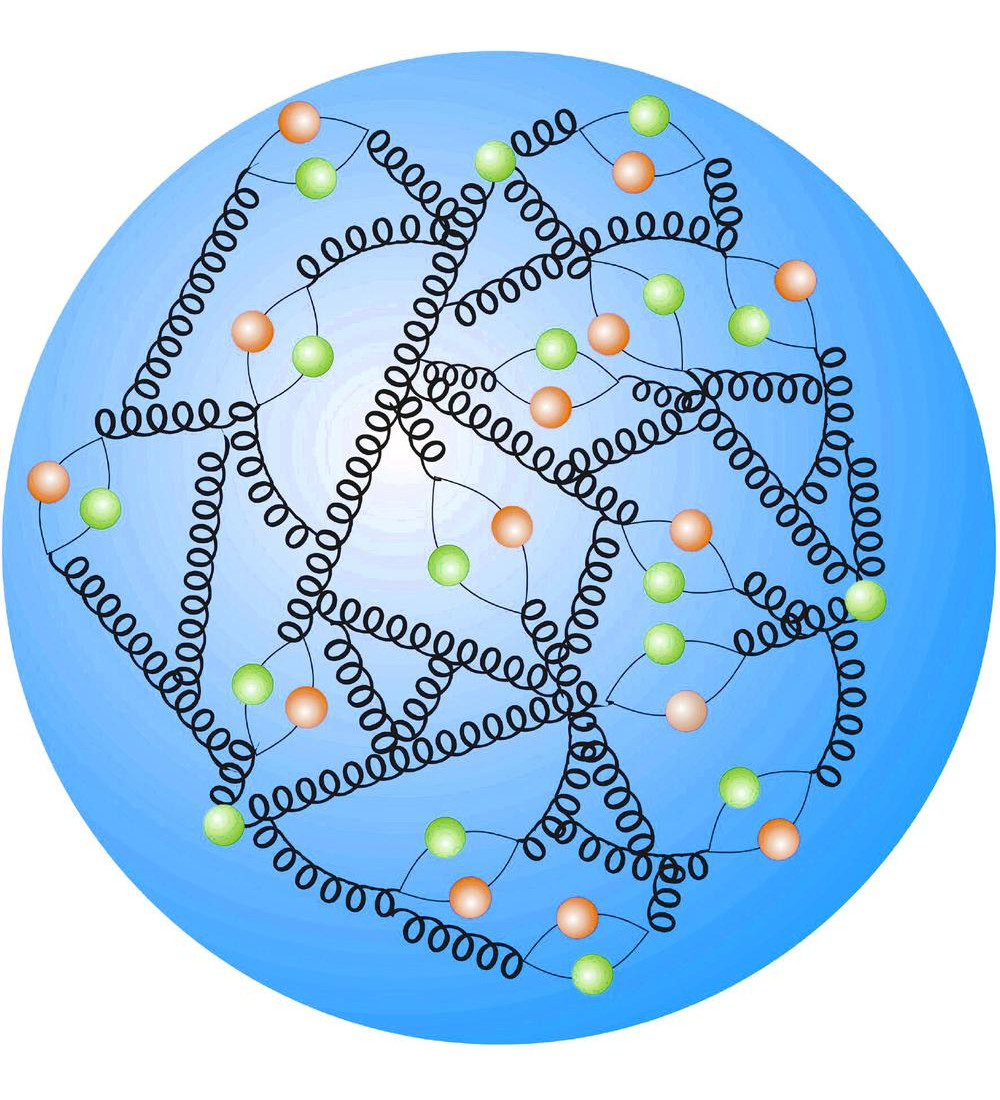
\includegraphics[width=0.30\textwidth]{figs/theory/proton_structure.jpg}
    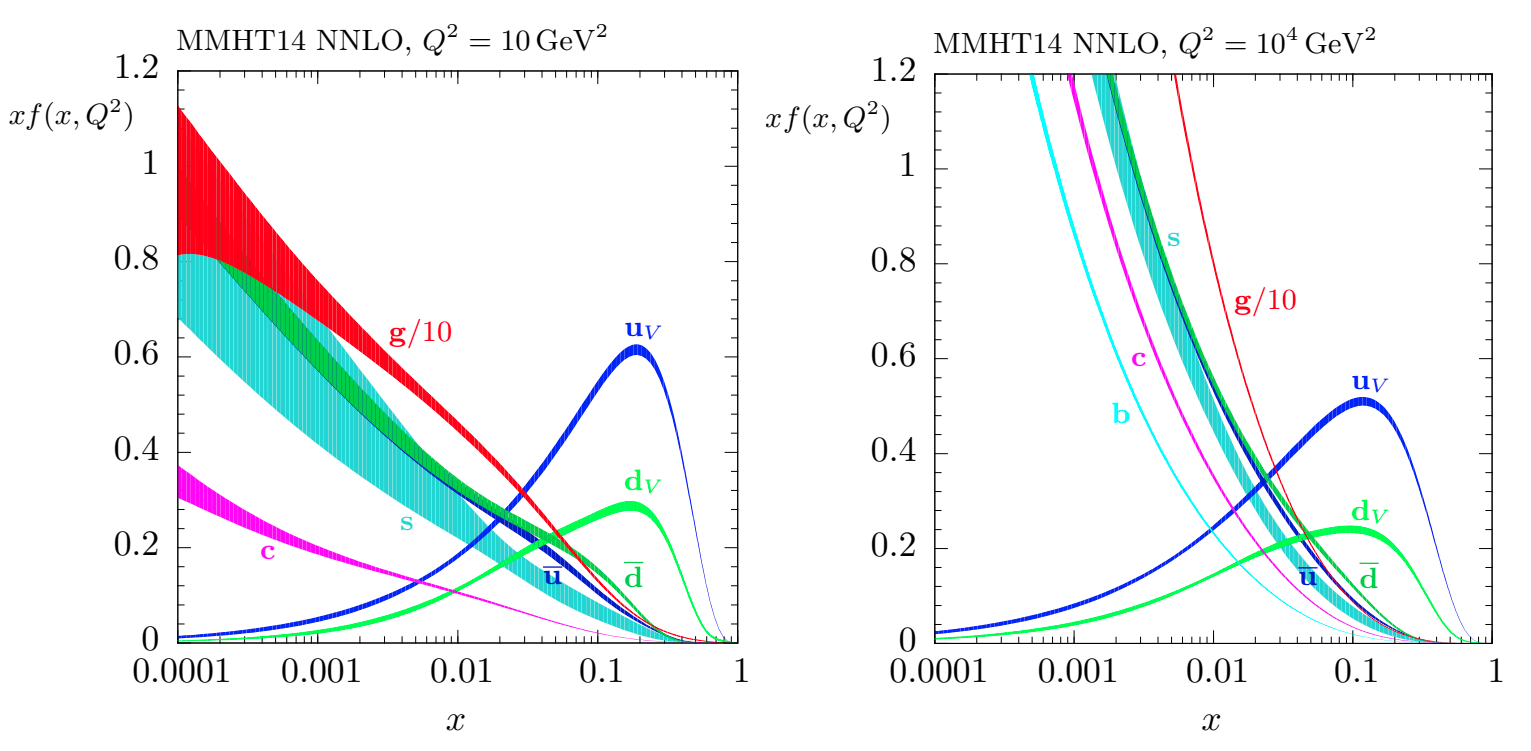
\includegraphics[width=0.66\textwidth]{figs/theory/pdfs.png}
    \caption{On the left, an illustration of the internal structure of the proton (image from~\cite{proton_image}).
      Gluons and quark-antiquark pairs constantly pop in and out of existence.
      The right two plots show MMHT2014 NNLO proton parton distribution functions,
      for momentum transfer scales $Q^2=10\GeV^2$ (center) and
      $Q^2=10^4\GeV^2$ (right). The quantity $x$ is the
      fraction of proton momentum carried by the parton.
      (Image from~\cite{pdfs})
            }
    \label{fig:pdfs}
  \end{center}
\end{figure}


When two protons collide, then, collisions can happen between any combination of valence
quarks and sea quarks/gluons. The higher the collision energy, the smaller the distance
scale probed and the more ``visible'' the sea quarks/gluons become.
This is quantified in what are called ``parton distribution functions'' (PDFs),
which are probability densities of finding a particular particle with longitudinal
momentum fraction $x$, given an energy scale $Q^2$. Examples are shown in 
Fig.~\ref{fig:pdfs} for $Q^2=10\GeV^2$ and $10^4\GeV^2$. One sees that the
PDFs for valence $u$ and $d$ quarks peak near one, as these are disproportionately
likely to carry a significant fraction of the proton's momentum.
The sea quarks and gluons peak lower, and become more prominent at higher $Q^2$.
These PDFs must be taken into account when computing cross sections for the various
$pp$ production processes.

\begin{figure}[htp]
  \addtolength{\abovecaptionskip}{5mm}
  \centering
  \vskip5mm
  \begin{fmffile}{feynman_diagrams/z_nunu}
  \begin{fmfgraph*}(40,25)
    \fmfleft{i2,i1}
    \fmfright{o2,o1}
    \fmftop{t}
    \fmf{phantom}{i1,v1,i2}
    \fmf{phantom}{o1,v2,o2}
    \fmf{phantom}{v1,v2}
    \fmffreeze
    \fmf{fermion}{i1,g}
    \fmf{plain,tension=2.8}{g,v1}
    \fmf{fermion}{v1,i2}
    \fmf{gluon,tension=0}{t,g}
    \fmf{boson,label=$Z$,label.side=right}{v1,v2}
    \fmf{fermion}{o2,v2,o1}
    \fmflabel{$q$}{i1}
    \fmflabel{$\bar{q}$}{i2}
    \fmflabel{$\bar{\nu}$}{o2}
    \fmflabel{$\nu$}{o1}
  \end{fmfgraph*}
\end{fmffile}
 \hskip1cm
  \begin{fmffile}{feynman_diagrams/wlnu}
  \begin{fmfgraph*}(50,25)
    \fmfleftn{i}{2}
    \fmfrightn{o}{4}
    %particelle entranti
    \fmf{fermion}{i1,v1}
    \fmf{fermion}{v2,i2}
    \fmflabel{$\bar{q}_i$}{i2}
    \fmflabel{$q_j$}{i1}
    %mediatore
    \fmf{fermion}{v1,v2}
    %%% produzione Z
    \fmf{photon,label=$W$}{v2,v4}
    % produzione l l
    \fmf{fermion}{v4,o4}
    \fmf{fermion}{o3,v4}
    \fmflabel{$\ell$}{o3}
    \fmflabel{$\nu_\ell$}{o4}
    %%% produzione glume
    \fmf{gluon}{v1,v3}
    %produzione b b
    \fmf{fermion}{v3,o2}
    \fmf{fermion}{o1,v3}
    \fmflabel{$q_k$}{o2}
    \fmflabel{$\bar{q}_l$}{o1}
  \end{fmfgraph*}
\end{fmffile}
 \\ \vskip2cm
  \begin{fmffile}{feynman_diagrams/multijet}
  \begin{fmfgraph*}(50,25)
    \fmfleft{i2,i1}
    \fmfright{o3,o2,o1}
    \fmftop{t}
    \fmf{phantom}{i1,v1,i2}
    \fmf{phantom}{o1,v2,o3}
    \fmf{phantom}{v1,v2}
    \fmffreeze
    %\fmfshift{5 left}{i1}
    %\fmfshift{5 up}{i1,t}
    \fmf{gluon,tension=0.8}{g,i1}
    \fmf{fermion}{v1,g}
    \fmf{fermion}{i2,v1}
    \fmf{fermion,tension=0}{g,t}
    \fmf{gluon}{v1,v2}
    \fmf{fermion}{o3,v2}
    \fmf{fermion}{v2,g2}
    \fmf{plain,tension=2.0}{g2,o1}
    \fmf{gluon,tension=0}{g2,o2}
    \fmflabel{$g$}{i1}
    \fmflabel{$q$}{i2}
    \fmflabel{$q$}{t}
    \fmflabel{$\overline{q'}$}{o3}
    \fmflabel{$q'$}{o1}
    \fmflabel{$g$}{o2}
  \end{fmfgraph*}
\end{fmffile}
 \hskip1cm
  \begin{fmffile}{feynman_diagrams/tth}
  \begin{fmfgraph*}(40,25)
    \fmfleft{d,i1,d,d,i3,d}
    \fmfright{o1,d,o2,d,o3}
    \fmf{gluon,tension=1.2}{i1,v1}
    \fmf{gluon,tension=1.2}{v3,i3}
    \fmf{fermion}{o1,v1}
    \fmf{fermion}{v3,o3}
    \fmf{phantom,tension=0.3}{v1,v3}
    \fmffreeze
    \fmf{fermion}{v1,v2,v3}
    \fmf{dashes,tension=1.3}{v2,o2}
    \fmflabel{$g$}{i3}
    \fmflabel{$g$}{i1}
    \fmflabel{$t$}{o3}
    \fmflabel{$\bar{t}$}{o1}
    \fmflabel{H}{o2}
  \end{fmfgraph*}
\end{fmffile}
 \\ \vskip1.5cm
  \begin{fmffile}{feynman_diagrams/ttbar}
  \begin{fmfgraph*}(77,47)
    \fmfleft{d,i2,d,i1,d}
    \fmfright{o1,d,o2,d,o3,d,o4,d,o5,d,o6}
    \fmf{gluon,tension=1.5}{i1,v1}
    \fmf{gluon,tension=1.5}{i2,v1}
    \fmf{gluon,tension=3}{v1,v2}
    \fmf{fermion,tension=2,label=$\bar{t}$,label.side=left,label.dist=7}{v4,v2}
    \fmf{fermion,tension=2,label=$t$,label.side=left,label.dist=7}{v2,v3}
    \fmf{fermion}{o3,v4}
    \fmf{fermion}{v3,o4}
    \fmf{boson,label=$W^-$,label.side=right,label.dist=3}{v4,v5}
    \fmf{fermion}{o1,v5,o2}
    
    \fmf{boson,label=$W^+$,label.side=left,label.dist=3}{v3,v6}
    \fmf{fermion}{o6,v6,o5}
    
    \fmflabel{$\mu^+$}{o1}
    \fmflabel{$\nu_\mu$}{o2}
    \fmflabel{$\bar{b}$}{o3}
    \fmflabel{$b$}{o4}
    \fmflabel{$u$}{o5}
    \fmflabel{$\bar{d}$}{o6}
  \end{fmfgraph*}
\end{fmffile}
 \vskip0.5cm
    \caption{Diagrams of the production of a few important processes at $pp$ colliders.
      From left-to-right, top-to-bottom: a SM monojet signature, caused by a $Z$ decaying
      invisibly to $\nu\bar{\nu}$ and an initial quark radiating a gluon;
      \wjets production, in this case $W\to\ell\nu$ plus two jets;
      QCD multijet production, in this case with three quark jets and one gluon jet;
      $\ttbar H$ production; and a full \ttbar decay chain, where one of the $W$'s from
      a top decays leptonically and one decays hadronically, producing a final state
      with a prompt lepton, missing energy, and four jets, two of which are b jets.
            }
    \label{fig:lhc_diagrams}
\end{figure}

Now knowing that collisions can happen between any valence quarks or sea quarks
and gluons, we can put together the vertices presented in Sec.~\ref{sec:fund_int}
to make diagrams of various interesting final states possible to achieve
at $pp$ colliders. A few examples are shown in
Fig.~\ref{fig:lhc_diagrams}.

First, in the top left, is the production of a $Z$ boson. From our PDFs,
we know that the most likely quarks are a $u$ valence quark and a $\bar{u}$
sea quark, followed by a $d$ valence quark and a $\bar{d}$ sea quark.
Also note that since one is a valence quark and one is a sea quark, there
is likely a momentum imbalance, so the entire event will
be boosted in the longitudinal direction. The transverse momentum, however,
will be very close to 0.

In this case we have shown the $Z$ decaying into neutrinos, which will be
invisible to the detector. The $Z$ can also decay into charged leptons,
giving the Drell-Yan process, or quarks. We have also shown a gluon
radiating off one of the initial state quarks, called ``initial state radiation'',
or ISR.

Now the strong force is a short range force, and energy actually increases without bound
as a colored particle is separated from its bound state (in contrast to electromagnetism, 
where the energy goes to 0 at infinite separation). This means that isolated quarks and gluons
cannot exist (called \textit{color confinement}), 
as eventually it becomes energetically favorable to produce new quark-antiquark
pairs. In hadron colliders, a high-energy quark or gluon thus undergoes a process called
\textit{hadronization}, in which it produces a narrow cone of hadrons called a jet as it
is expelled from the collision point. The signature represented by the first diagram in
Fig.~\ref{fig:lhc_diagrams} is thus a ``monojet'': a single high-energy jet, recoiling against
invisible energy from the neutrinos from $Z$ decay.

Continuing to the right in Fig.~\ref{fig:lhc_diagrams}, we have
the production of a $W$ boson which decays to a $\ell\nu$ pair.
We've also shown an ISR gluon splitting into two quarks, which
show up as two jets. This diagram thus represents a leptonic \wjets
event.

Next in the middle left  is a generic diagram representing QCD multijet production,
the most common type of event at hadron colliders. 
In this case we have an interaction between a valence quark and sea
gluon, which results in a final state of three quarks and a gluon,
giving a four jet event. By tacking on more quark/gluon vertices to this
or similar diagrams, we can create events with any number of jets. Dijets
are the most common type of event, and the rate falls exponentially
with the number of jets (each jet reduces the cross section roughly by
a factor of 10).

In the middle right we have a diagram representing $\ttbar H$ production
from two gluons. This will not be very relevant for the analysis in this
dissertation, but it is a important process under study at the LHC to
better understand the nature of the Higgs boson and its coupling to top quarks.

\begin{figure}[t]
  \begin{center}
    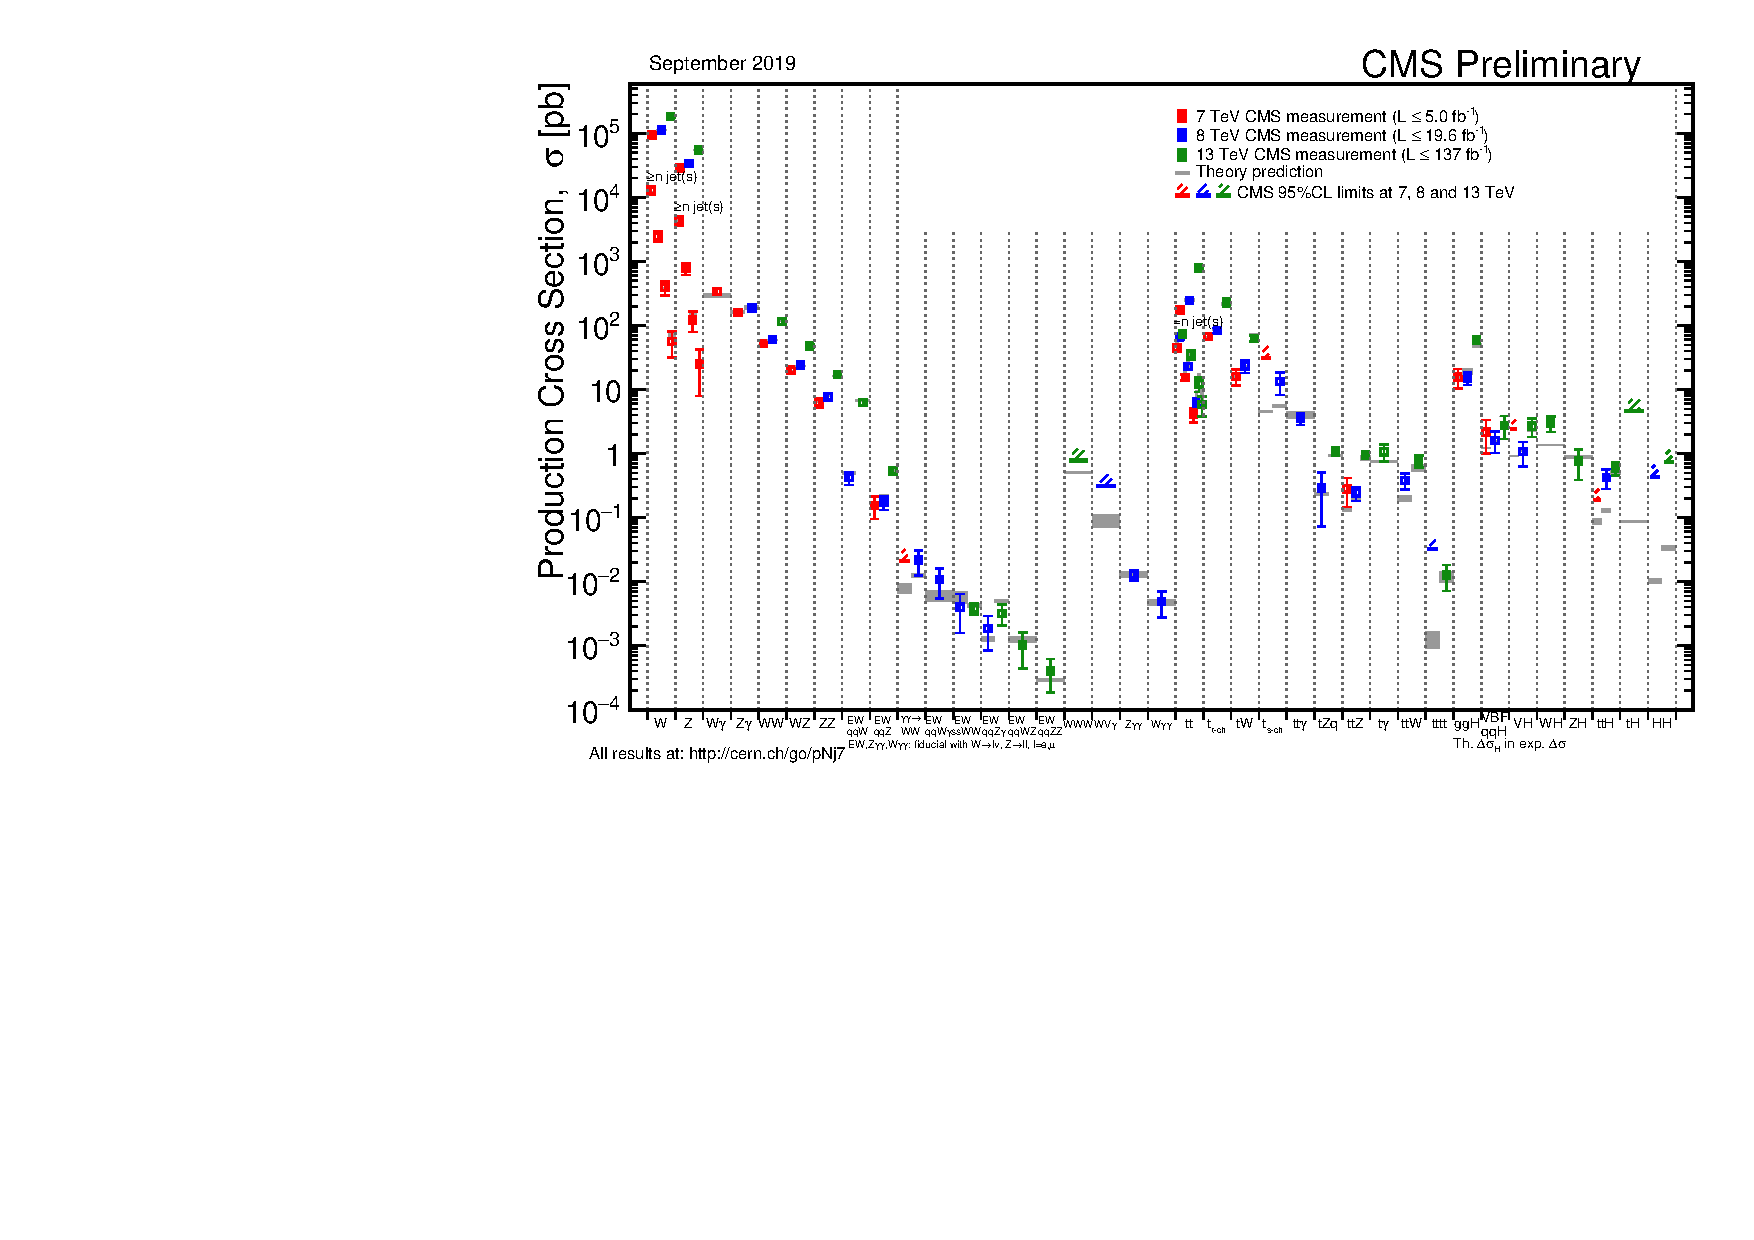
\includegraphics[width=1.00\textwidth]{figs/theory/cms_xsecs.pdf}
    \caption{Summary of SM production cross sections measured at CMS, compared to
      values predicted from theory. (Image from~\cite{CMS:xsecs})
            }
    \label{fig:cms_xsecs}
  \end{center}
\end{figure}

And finally, the bottom diagram shows the production of a $\ttbar$ pair through
gluon-gluon fusion. Top quarks are the only quarks that do not undergo hadronization,
since they decay too quickly due to their very high mass. Since the on-diagonal
$V_{tb}$ element of the CKM matrix is very nearly one, top quarks decay nearly 100\% of the
time to a $W$ boson and $b$ quark. The $b$ quarks hadronize into $b$ jets (identifiable
due to the long lifetime of $B$ hadrons), and the $W$ bosons can decay either
hadronically (70\% of the time) or leptonically (10\% each to $e$, $\mu$, $\tau$).

Using the PDFs, theorists have computed cross sections for a huge variety of SM processes
at the LHC. These have then been measured by the various experiments. A summary plot
from CMS is shown in Fig.~\ref{fig:cms_xsecs}; one sees that the experimentally measured
cross sections agree well with the theoretical predictions in all cases.

Theorists can also calculate the cross sections of hypothetical BSM production modes,
such as SUSY. Fig.~\ref{fig:susy_xsecs} shows the cross sections for the pair production
of gluinos and squarks at $\sqrt{s}=13\TeV$. One sees that the cross section exponentially
falls with sparticle mass.


\begin{figure}[ht]
  \begin{center}
    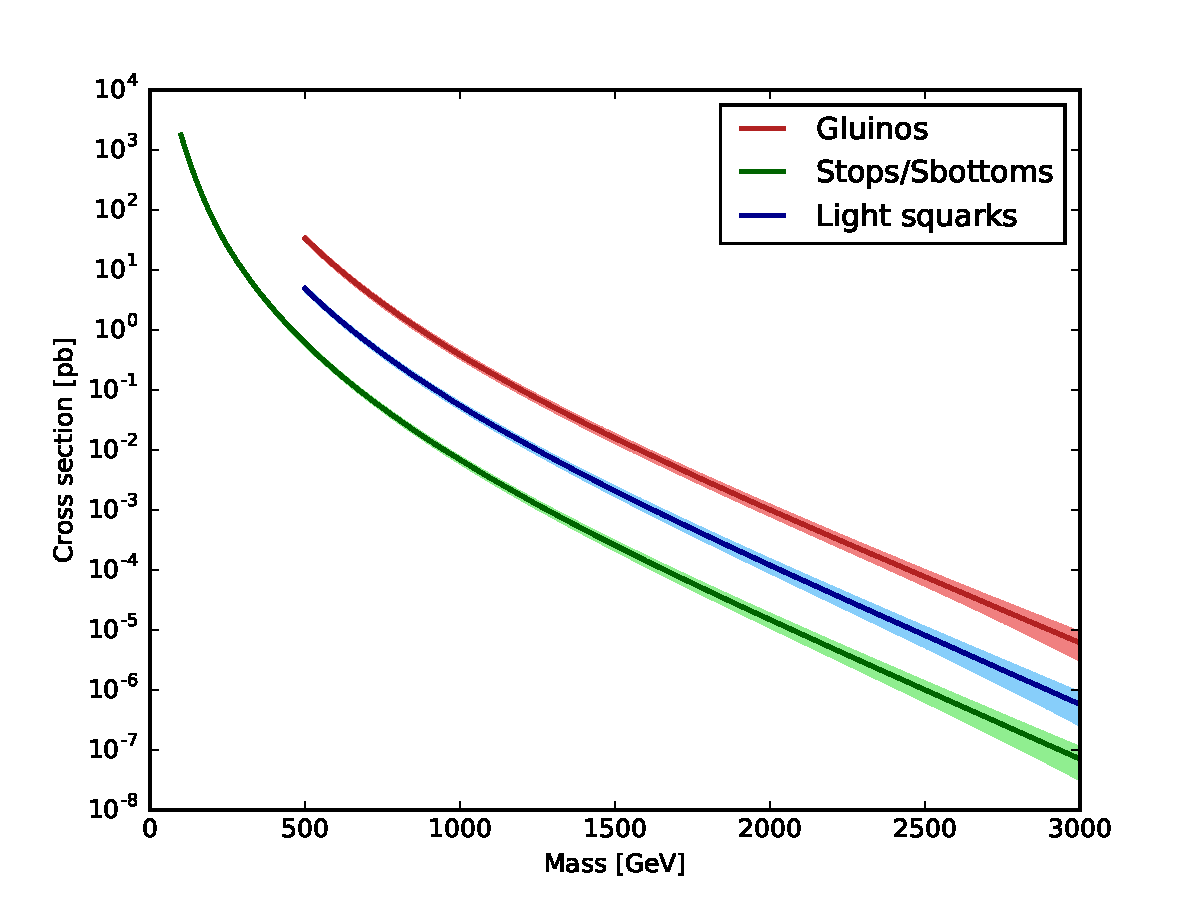
\includegraphics[width=0.60\textwidth]{figs/theory/susy_xsecs.pdf}
    \caption{Cross sections for pair production of SUSY particles at the LHC at $\sqrt{s}=13\TeV$,
      computed at NNLO(approx)+NNLL order~\cite{Beenakker:nnll} and assuming squarks and gluinos are decoupled. 
      The $x$ axis is the mass of the relevant particle.
      The light squark cross section assumes 8-fold degeneracy between left- and right-handed
      $\SQu,\;\SQd,\;\SQs,\;\text{and}\;\SQc$ squarks.
            }
    \label{fig:susy_xsecs}
  \end{center}
\end{figure}
